\documentclass[11pt,oneside]{thesis}
\usepackage{subfigure}
\usepackage[linesnumbered,lined,titlenumbered,ruled]{algorithm2e}
\usepackage{amsmath}
\usepackage{amssymb}
\usepackage{amsbsy}
\usepackage{mathpazo}
\usepackage{float}

%\floatstyle{ruled}
%\restylefloat{table}

\renewcommand{\tablename}{Tabla}
%\dontprintsemicolon

\title{Título}
\author{Autor}
\advisor{Tutores}
\degree{Grado}
\university{Universidad}
\faculty{Facultad}
\date{Fecha}
\logo{graphics/university_logo}
\makenomenclature

\renewcommand{\vec}[1]{\boldsymbol{#1}}
\newcommand{\diff}[1]{\ensuremath{\mathrm{d}#1}}

\begin{document}

\frontmatter
\maketitle

%===================================================================================
% Chapter: Phrase
%===================================================================================

\begin{phrase}[4.2in]
	Dedicado a mis padres, Ramón y Amparo, quienes han batallado a mi lado incansablemente y de forma incondicional durante estos $23$ años de vida y $18$ años de estudio.\\
	A Julio, mi hermano, quien siempre ha estado certero con sus consejos y apoyándome en todo lo que he necesitado fuera y dentro del ámbito educacional.\\
	A Odalmis, mi novia, prometida y próximamente esposa, hemos cursado los buenos y malos momentos en en estos últimos $4$ años y ha estado siempre presente para dar un consejo o apoyo cuando lo necesito.\\
	A todo aquel que, sin importar si fue un simple \doublequote{buenos días}, una charla pasajera o esporádica o una larga amistad de años, intervino en mi vida para hacer de mí lo que soy hoy.
\end{phrase}
thanks
%===================================================================================
% Chapter: Supervisor Opinion
%===================================================================================

\begin{opinion}
	La representación de conocimiento se ha convertido en un área de investigación muy activa en los últimos años, motivada tanto por la disponibilidad masiva de nuevos recursos, como por la necesidad de hacer computacionalmente tratable el volumen de datos producidos diariamente. Su relevancia en tareas más amplias, como el descubrimiento automático de conocimiento, la vuelven un área crucial para el desarrollo de varios sectores de la sociedad. En el dominio médico, la aplicación de estas técnicas se vuelve especialmente interesante, ya que procedimientos de inferencia sobre una base de conocimiento puede potencialmente ayudar a diseñar nuevos tratamientos para combatir enfermedades aún no resueltas. En este marco se desarrolla la tesis de licenciatura de José Ariel Romero Costa, con quien pude trabajar este último año en el diseño y validación de un algoritmo para la construcción de ontologías a partir de textos anotados. Esta tesis da continuidad a una línea de investigación que se ha venido desarrollando en la facultad en los últimos años ligada al descubrimiento de conocimiento.

	La propuesta de José consiste en un algoritmo para la creación automática de ontologías a partir de una colección anotada de documentos. El sistema utiliza el esquema de anotación del \emph{eHealth-KD Challenge} que ha sido empleado en dos competencias internacionales de extracción de conocimiento, en el marco de los eventos \emph{IberLEF 2019} e \emph{IberLEF 2020}. El trabajo conllevó reconstruir un corpus de texto de Medline sobre el que identificar y reordenar las oraciones del corpus anotado. A partir de las entidades y relaciones señaladas en el texto, se realiza un proceso de normalización con el objetivo de unificar aquellas entidades que difieren sintácticamente pero comparten la misma semántica. La tesis presenta un procedimiento para organizar la información recogida en múltiples oraciones, formando una base de conocimiento que integra las distintas instancias de anotaciones mencionadas entre colecciones. La representación final obtenida constituye un paso de avance en la formalización del esquema de anotación, y sienta las bases para futuros procesos de inferencia.

	Durante el desarrollo de la tesis José demostró independencia y creatividad para lidiar con los problemas encontrados. Tuvo que dominar conceptos y tecnologías del estado del arte, con muchas de las cuales no tuvo contacto durante la carrera. Los problemas que hubo de resolver le servirán de aprendizaje para su desarrollo futuro. El proceso de investigación e implementación desarrollado por José queda recogido en un documento de tesis que avala la capacidad adquirida para presentar resultados de investigación de forma concisa y coherente. Todo esto lo han realizado a la par de las actividades docentes, como estudiante de pregrado y como alumno ayudante de la asignatura \emph{Programación}, donde ha sabido asumir con éxito todas las responsabilidades y retos.

	José ha sido alumno ayudante desde su tercer año en la carrera, tiempo que pude compartir con él directamente en clases y en las reuniones del colectivo. En esos años he podido comprobar su interés y dedicación por la asignatura y otros temas relacionados. Este último ejercicio demuestra que ya ha adquirido la madurez necesaria para desarrollar proyectos de alta complejidad con calidad y esmero. Como tutor, estoy complacido por los resultados obtenidos, y por el trabajo realizado con José, que aunque no estuvo exento de obstáculos, logró superar los desafíos. Por estos motivos estoy convencido de que José será un excelente profesional de la Ciencia de la Computación.

	\vspace{1cm}
	\begin{flushright}
		\emph{MSc. Juan Pablo Consuegra Ayala}\\
		Facultad de Matemática y Computación\\
		Universidad de La Habana
	\end{flushright}
\end{opinion}
%===================================================================================
% Chapter: Abstract (english)
%===================================================================================
\ChapterOutOfToc{Abstract}\label{chapter:abstract_english}
%===================================================================================

\hyphenation{de-fined}
\hyphenation{ex-posed}
\hyphenation{knowl-edge}
\hyphenation{scheme}

In recent years there has been an increase in the development of techniques for automatic knowledge discovery from documents written on natural language. Automatic processing provides the possibility to analyze collections of information containing a large number of texts. In the medical field, the rise of these technologies is significantly special, because it allows taking advantage of the huge amount of data available for it and improve research on this area, which is really important to society. These techniques tend to rely on annotated corpus, and they are a scarce resource. This becomes a critical fact in Spanish language, where the existing amount of them is very low and from a less general domain.

In this study, a general-purpose annotation model is defined to capture the most relevant semantic features contained in text documents. Also, an ontology scheme is presented and used for automatic knowledge extraction. A theoretical step by step implementation of a computational algorithm aiming to build a knowledge graph from an annotated corpus and following the rules of the previously defined ontology is also proposed. Finally, the evaluation and validation process is exposed, as well as statistics results.

The results achieved demonstrate that knowledge discovery constitutes an active research field, where machine learning techniques can be applied achieving positive results. The verification and comparison of a specific knowledge graph built from the proposals provided in this investigation against the learning and interpretation skills of a group of experts on the same field is proposed. Also, the continuation of this research line is suggested, aiming to improve the effectiveness of the proposals given and their application in other domains.
%===================================================================================
% Chapter: Contents
%===================================================================================

\tableofcontents
\listoffigures
\listoftables

\mainmatter
	
%===================================================================================
% Chapter: Introduction
%===================================================================================
\Chapter*{Introducción}\label{chapter:introduction}
%===================================================================================

\hyphenation{herra-mien-tas}
\hyphenation{corre-la-cio-nar-los}

El desarrollo tecnológico se ha exacerbado con el advenimiento cada vez mayor del uso del Internet y otros medios avanzados y efectivos que garantizan un mejor futuro para cuestiones importantes de la vida. Debido al continuo aumento del flujo informativo, se hace cada vez más necesaria la utilización de herramientas que permitan identificar, capturar y representar el conocimiento dentro de los sistemas de información, ya sea de dominio específico o de propósito general.

Para ello, ciencias avanzadas como la Ciencia de la Computación y de la Comunicación comprenden la ontología como la definición de conceptos y relaciones en algún dominio, de forma compartida y consensuada. Esta conceptualización debe ser representada de una manera formal, legible y utilizable por los ordenadores~\cite{ref:30}. Son creadas para limitar la complejidad de cualquier tema y para organizar la información. Es una medida eficaz en las soluciones de problemas comunes en la vida diaria, que debido a la sobreinformación no se podrían llevar a cabo de forma manual.

Otro de sus beneficios es el hecho de que permiten crear entendimiento compartido al unificar los diferentes puntos de vista. Esto sirve para facilitar la comunicación entre los actores implicados en la construcción de sistemas de información referidos al dominio. Además, permiten el reuso del conocimiento del tema, pues sirve de base ya creada para posteriores investigaciones. También facilitan la recuperación, integración e interoperatividad entre fuentes de conocimiento heterogéneas. Con ellas se provee una base para la representación del conocimiento del dominio y ayudan a identificar las categorías semánticas del mismo~\cite{ref:1}.

Surge entonces el creciente interés de estudiar técnicas para el descubrimiento automático de conocimiento. El procesamiento automático trae consigo la posibilidad de analizar colecciones masivas de información. Sin embargo, la mayor parte de estas colecciones almacenan la información disponible en documentos textuales escritos en lenguaje natural. La naturaleza en que se expresa la información y su estructura semántica poco unificada se vuelven la principal fuente de retos de dicho procesamiento.

En la actualidad, las ontologías se están aplicando en áreas heterogéneas. Entre ellas se encuentran la búsqueda de información, el comercio electrónico, configuraciones de aplicaciones o productos. Además, todo sitio web grande debería usarlas, al menos para organización y navegación~\cite{ref:31}. También se están utilizando para el desarrollo de mecanismos que faciliten la comunicación entre las personas y las máquinas por medio del lenguaje natural~\cite{ref:2}.

En el contexto de la salud y la medicina las ontologías adquieren particular interés, debido a que se están utilizando cada vez más para la solución de disímiles tareas, como la recuperación de información y la búsqueda de respuestas en fragmentos de texto que resuelven preguntas. Diariamente se publican muchos artículos médicos y se hace imposible acceder a todos y obtener conocimiento sobre las novedades médicas y las herramientas que se van desarrollando para solucionar las enfermedades o los problemas de la salud de manera general.

La extracción automática de conocimiento proveería de una herramienta para asistir el desarrollo en esta área a partir de la normalización e integración de los resultados encontrados. Una vez extraído y representado el conocimiento computacionalmente, procesos de inferencia permitirían el descubrimiento de nuevo conocimiento. Ejemplo de esto es el constante descubrimiento de nuevas interacciones entre medicamentos, proteínas y genes. Un sistema de descubrimiento de conocimiento posibilitaría la detección automática de
nuevas relaciones entre ellos, y por ende, el descubrimiento de nuevas causas de enfermedades, síntomas y tratamientos.\\

Algunas de las razones principales para el desarrollo de una ontología son:

\begin{itemize}
	\item[•] Compartir conocimiento de la estructura de la información entre investigadores y/o usuarios.
	\item[•] Permitir la reutilización del conocimiento del dominio.
	\item[•] Hacer explícitas las suposiciones o conocimientos a priori del dominio.
	\item[•] Separar el conocimiento explícito del dominio del conocimiento implícito operacional.
	\item[•] Analizar el conocimiento del dominio.
\end{itemize}

\textit{Compartir conocimiento de la estructura de la información entre investigadores y/o usuarios} es uno de los objetivos comunes en el desarrollo de ontologías~\cite{ref:4,ref:10}. Por ejemplo, si varios sitios web diferentes entre sí contienen información médica o proporcionan servicios médicos de comercio electrónico, y estos comparten y publican la misma ontología subyacente de los términos que utilizan, los agentes informáticos pueden extraer y agregar información de los mismos. Además, estos últimos pudieran utilizar dicha información para responder consultas de los usuarios o como datos de entrada para otras aplicaciones.

\textit{Permitir la reutilización del conocimiento del dominio} fue una de las fuerzas impulsoras detrás del reciente aumento de la investigación ontológica. Por ejemplo, los modelos para muchas áreas diferentes deben representar la idea de tiempo. Esta representación incluye, entre otros, las nociones de intervalos, puntos y medidas relativas a este. Si un grupo de investigadores desarrolla tal ontología en detalle, otros pueden simplemente reutilizarla para sus dominios. Además, si se necesita construir una grande, se pueden integrar varias ya existentes que describan partes específicas de la rama deseada. También se puede reutilizar una de propósito general, como UNSPSC, y extenderla para describir el área de interés.

\textit{Hacer explícitas las suposiciones o conocimientos a priori del dominio} hace posible cambiarlas fácilmente si cambian las ideas tenidas de antemano en este tema. Los supuestos de \textit{codificación rígida} (del inglés \textit{hard-coding}) sobre el mundo hechos en lenguajes de programación hacen que estas no solo sean difíciles de encontrar y comprender, sino también de cambiar, en particular para alguien sin experiencia en el ámbito computacional. Además, las especificaciones explícitas del conocimiento del dominio son útiles para los nuevos usuarios que deben aprender qué significan los términos de este.

\textit{Separar el conocimiento explícito del dominio del conocimiento implícito operacional} es otro uso común de las ontologías. Se puede describir la tarea de configurar un producto a partir de sus componentes, de acuerdo con una especificación requerida e implementar un programa que realice esta configuración independientemente del producto~\cite{ref:11}. Seguido de esto, se puede desarrollar una ontología de componentes y características de los ordenadores personales y aplicar el algoritmo para configurar uno de ellos a medida~\cite{ref:12}.

\textit{Analizar el conocimiento del dominio} es posible una vez se disponga de una especificación declarativa de los términos. El análisis formal de estos es extremadamente valioso cuando se intenta reutilizar ontologías existentes y ampliarlas~\cite{ref:13}.

\noindent\textbf{\large Problemática}

En disímiles ocaciones, es necesaria la lectura de un amplio grupo de documentos con gran cantidad de páginas para poder tener conocimiento acerca de algún tema. Incluso algunas veces la información leída no es relevante para lo que se desea, y por tanto, fue una inversión de tiempo en vano. Las ontologías, por otra parte, aceleran en gran medida este proceso, pues el análisis y representación de uno o más corpus en un grafo de conocimiento es cuestión de segundos. Esto posibilita posteriormente, buscar la información deseada a través de consultas realizadas a un sistema computacional.

Para diseñar una ontología no existe una única forma o metodología correcta a emplear y tampoco es objetivo de este estudio definir una. Con esta investigación se busca dar solución al problema de representar un corpus de documentos anotados como base de conocimiento, por medio de una ontología. Para ello es necesaria la definición de la propia ontología a usar y un algoritmo computacional que posibilite la realización de este proceso.

La generación de ontologías es un proceso que de ser realizado de forma manual, toma demasiado tiempo y esfuerzo. Además, en aras de completar la construcción de una base de conocimientos medianamente buena o buena, es necesario involucrar expertos en el dominio. Por otra parte, estas restricciones imposibilitan la realización de una ontología para todos los posibles corpus de estudio. En cambio, con esta investigación se busca realizar este proceso de forma totalmente automática, sin la necesidad tener conocimiento previo del dominio y tras la espera de unos pocos segundos puede verse el resultado de la ontología construida.

Este problema lleva implícito el procesamiento de lenguaje natural, pues en este están escritos los corpus de documentos que serán usados. Además, el campo de estudio de la generación automática de ontologías es relativamente moderno. Este conjunto de aspectos lo hace ser un problema interesante. Es por esto que es el objetivo de esta investigación.

En esta investigación, además de definir un esquema de ontología de propósito general, se lleva a cabo la realización de una base de conocimiento mediante la utilización de un corpus de dominio médico extraído de \textit{Medline}~\cite{ref:3}.\\

\noindent\textbf{\large Objetivos}

La investigación se plantea como objetivo general definir un diseño de ontología de propósito general que sea capaz de representar el conocimiento descrito en uno o más corpus anotados.

Para darle solución al objetivo general es necesaria la implementación de un algoritmo computacional capaz de representar uno o más corpus de documentos anotados como un grafo de conocimiento que responde a las reglas establecidas por la ontología propuesta.

Se proponen los siguientes objetivos específicos:
\begin{itemize}
	\vspace{-0.27cm}
	\item[•] Estudiar los esquemas de anotación y corpus usados en diversas tareas de extracción del conocimiento.
	\vspace{-0.27cm}
	\item[•] Definir un esquema conceptual de anotación para la representación de los rasgos semánticos más relevantes en textos escritos en lenguaje natural.
	\vspace{-0.27cm}
	\item[•] Definir un formato de anotación de archivos para el esquema conceptual previamente definido.
	\vspace{-0.27cm}
	\item[•] Diseñar una propuesta de ontología donde se pueda representar un corpus de documentos escritos en lenguaje natural.
	\vspace{-0.27cm}
	\item[•] Implementar un algoritmo computacional para representar un corpus anotado como grafo de conocimiento a través de dicha ontología.
	\vspace{-0.27cm}
	\item[•] Implementar un marco experimental para la evaluación de la propuesta de solución.
\end{itemize}

\noindent\textbf{\large Organización de la tesis}

El contenido de la tesis se organiza de la siguiente forma. El capítulo \ref{chapter:automatic_generation_of_ontologies} introduce los principales conceptos relacionados con las ontologías y la extracción y representación de conocimiento. En este capítulo, además, se analizan los principales corpus y representaciones semánticas existentes en la literatura. El capítulo \ref{chapter:annotation_model} describe un modelo de anotación de propósito general que busca capturar los rasgos semánticos más importantes en documentos de texto. En el capítulo \ref{chapter:proposed_solution} se presenta una propuesta para la creación de un grafo de conocimiento a través de un corpus anotado. En el capítulo \ref{chapter:analysis_of_results} se muestran los resultados alcanzados en esta investigación, y en función de estos, se discute la efectividad de cada uno de los elementos propuestos en la misma. La investigación finaliza presentando las conclusiones pertinentes y las recomendaciones para su continuidad y mejora.
\include{mainmatter/background}
%===================================================================================
% Chapter: Analysis of Results
%===================================================================================
\chapter{Análisis de Resultados}\label{chapter:analysis-of-results}
%===================================================================================
El esquema de anotación y el modelo ontológico presentado en este trabajo, y por tanto el grafo de conocimiento generado a partir de ellos, tienen como objetivo fundamental asistir en el desarrollo de sistemas de descubrimiento de conocimiento en documentos escritos en lenguaje natural.

En este capítulo, se presenta el marco experimental diseñado para comprobar la efectividad del esquema de anotación y el modelo ontológico descrito en el capítulo \ref{chapter:annotation_model} y de la propuesta de solución presentada en el capítulo \ref{chapter:proposed-solution}.

\section{Marco experimental}
En esta investigación solo se trabajará con los artículos del corpus de \textit{Medline} en español, estos son procesados para eliminar las marcas específicas de \textit{HTML}\footnote{Siglas en inglés de \textit{\textbf{H}yper\textbf{T}ext \textbf{M}arkup \textbf{L}anguage}, un lenguaje de marcado usado en la elaboración de páginas web.} y ser divididos en oraciones. Luego, las oraciones anotadas son mezcladas con sus respectivos artículos. Potencialmente, un artículo podrá no tener ninguna de sus oraciones anotadas o estar completamente anotado. Las tablas \ref{tab:stats_corpus} y \ref{tab:stats_annotated_corpus} muestran algunas estadísticas acerca de este corpus y de las oraciones anotadas pertenecientes al mismo.

Estos resultados son extraídos usando \textit{python} como lenguaje de programación y los paquetes \textit{nltk} y \textit{spacy} para el procesamiento del lenguaje natural.

\begin{table}[H]
	\begin{center}
		\begin{tabular}{lccc}
			\noalign{\hrule height 1pt}\\
			\vspace{-0.35in}\\
			\textbf{Métrica} & \textbf{\textit{Medline}} & \textbf{Anotado} & \textbf{\% anotado}\\
			\hline\\
			\vspace{-0.35in}\\
			Artículos & $1,013$ & $25^*$ & $\approx2.47$\\
			\hline\\
			\vspace{-0.35in}\\
			Oraciones & $12,830$ & $999$ & $\approx7.79$\\
			Promedio de oraciones por artículo & $\approx13$ & $\approx40$ & $\approx307.69$\\
			Menor cantidad de oraciones en un artículo & $2$ & $39$ & $1,950$\\
			Artículos con la menor cantidad de oraciones & $9$ & $1$ & $\approx11.11$\\
			Mayor cantidad de oraciones en un artículo & $65$ & $40$ & $\approx61.54$\\
			Artículos con la mayor cantidad de oraciones & $1$ & $24$ & $2,400$\\
			\hline\\
			\vspace{-0.35in}\\
			Palabras & $191,256$ & $14,529$ & $\approx7.6$\\
			Promedio de palabras por artículo & $\approx189$ & $\approx581$ & $\approx307.41$\\
			Promedio de palabras por oración & $\approx15$ & $\approx15$ & $100$\\
			Menor cantidad de palabras en un artículo & $33$ & $489$ & $\approx1,481.82$\\
			Artículos con la menor cantidad de palabras & $1$ & $1$ & $100$\\
			Menor cantidad de palabras en una oración & $1$ & $4$ & $400$\\
			Oraciones con la menor cantidad de palabras & $87$ & $1$ & $\approx1.15$\\
			Mayor cantidad de palabras en un artículo & $1,199$ & $671$ & $\approx55.96$\\
			Artículos con la mayor cantidad de palabras & $1$ & $1$ & $100$\\
			Mayor cantidad de palabras en una oración & $258$ & $46$ & $\approx17.83$\\
			Oraciones con la mayor cantidad de palabras & $1$ & $1$ & $100$\\
			\noalign{\hrule height 1pt}\\
		\end{tabular}

		\vspace{-0.1in}
		*\small{Esta cifra no son artículos en sí, sino archivos, los cuales pueden contener oraciones de varios artículos.}
		\caption[Estadísticas del corpus tomado de \textit{Medline} y del anotado]{Estadísticas del corpus tomado de \textit{Medline} y del anotado.}
		\label{tab:stats_corpus}
	\end{center}
\end{table}

\begin{table}[H]
	\begin{center}
		\begin{tabular}{lcc}
			\noalign{\hrule height 1pt}\\
			\vspace{-0.35in}\\
			\textbf{Métrica} & \textbf{Total}\\
			\hline\\
			\vspace{-0.35in}\\
			Oraciones & $999$\\
			\hline\\
			\vspace{-0.35in}\\
			Conceptos & $6,324$ & \% conceptos\\
			\quad \texttt{Concept} & $3,914$ & $\approx61.89$\\
			\quad \texttt{Action} & $1,661$ & $\approx26.27$\\
			\quad \texttt{Reference} & $213$ & $\approx3.37$\\
			\quad \texttt{Predicate} & $536$ & $\approx8.47$\\
			\hline\\
			\vspace{-0.35in}\\
			Relaciones & $5,925$ & \% relaciones\\
			\quad \texttt{Subject} & $859$ & $\approx14.5$\\
			\quad \texttt{Target} & $1,688$ & $\approx28.49$\\
			\quad \texttt{Domain} & $346$ & $\approx5.84$\\
			\quad \texttt{Argument} & $333$ & $\approx5.62$\\
			\quad \texttt{Is-a} & $570$ & $\approx9.62$\\
			\quad \texttt{Part-of} & $95$ & $\approx1.6$\\
			\quad \texttt{Same-as} & $124$ & $\approx2.09$\\
			\quad \texttt{Has-property} & $168$ & $\approx2.84$\\
			\quad \texttt{Causes} & $381$ & $\approx6.43$\\
			\quad \texttt{Entails} & $170$ & $\approx2.87$\\
			\quad \texttt{In-time} & $154$ & $\approx2.6$\\
			\quad \texttt{In-place} & $384$ & $\approx6.48$\\
			\quad \texttt{In-context} & $653$ & $\approx11.02$\\
			\hline\\
			\vspace{-0.35in}\\
			Atributos & $559$ & \% atributos\\
			\quad \texttt{Negated} & $160$ & $\approx28.62$\\
			\quad \texttt{Uncertain} & $262$ & $\approx46.87$\\
			\quad \texttt{Diminished} & $17$ & $\approx3.04$\\
			\quad \texttt{Emphasized} & $120$ & $\approx21.47$\\
			\noalign{\hrule height 1pt}
		\end{tabular}
		\caption[Estadísticas del corpus anotado]{Estadísticas del corpus anotado.}
		\label{tab:stats_annotated_corpus}
	\end{center}
\end{table}

\section{Resultados computacionales}
En la figura \ref{fig:out_degree_all_nodes} se evidencia una relación entre el grado de salida de los nodos y la cantidad de estos que tienen un grado específico. Esto representa la cantidad de relaciones como las explicadas en la sección \ref{section:relation_annotation} en las que el nodo es parte izquierda (referenciado a través de \texttt{Arg1}).
\begin{figure}[H]
	\begin{center}
		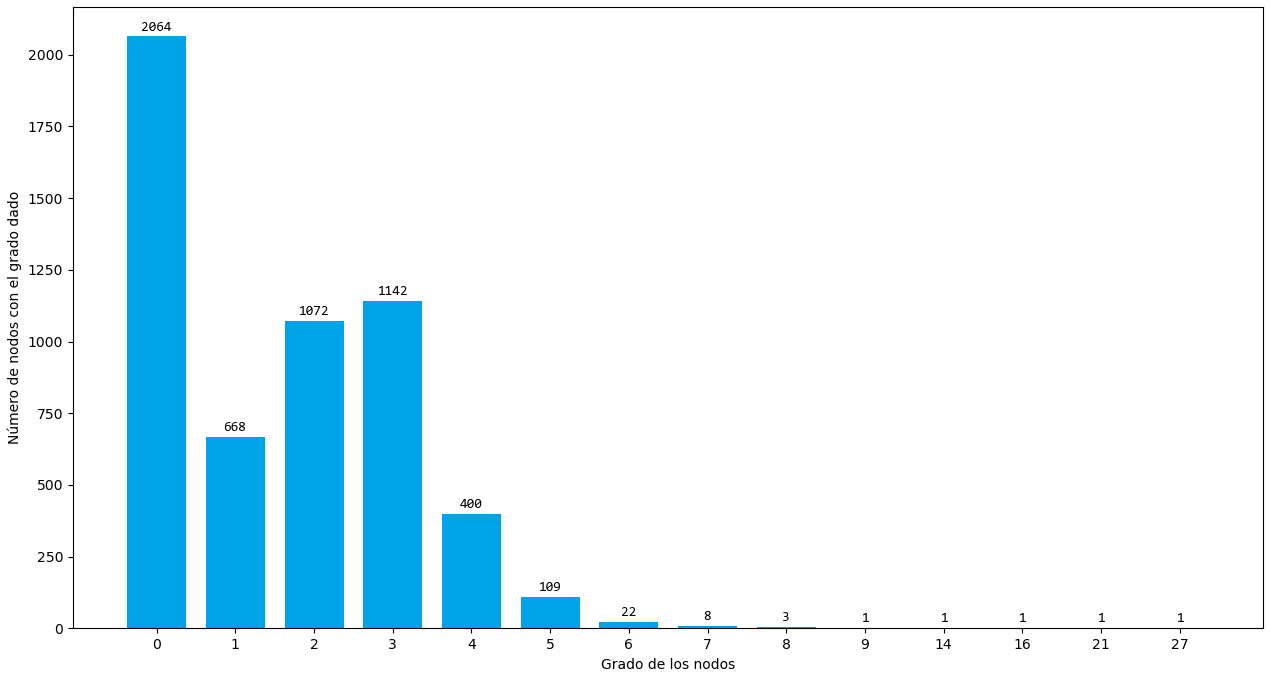
\includegraphics[width=\textwidth]{graphics/degree1.png}
		\caption[Grado de salida de los nodos del grafo]{Grado de salida de los nodos del grafo.}
		\label{fig:out_degree_all_nodes}
	\end{center}
\end{figure}

En la figura \ref{fig:in_degree_all_nodes} se evidencia una relación entre el grado de salida de los nodos y la cantidad de estos que tienen un grado específico. Esto representa la cantidad de relaciones como las explicadas en la sección \ref{section:relation_annotation} en las que el nodo es parte derecha (referenciado a través de \texttt{Arg2}).
\begin{figure}[H]
	\begin{center}
		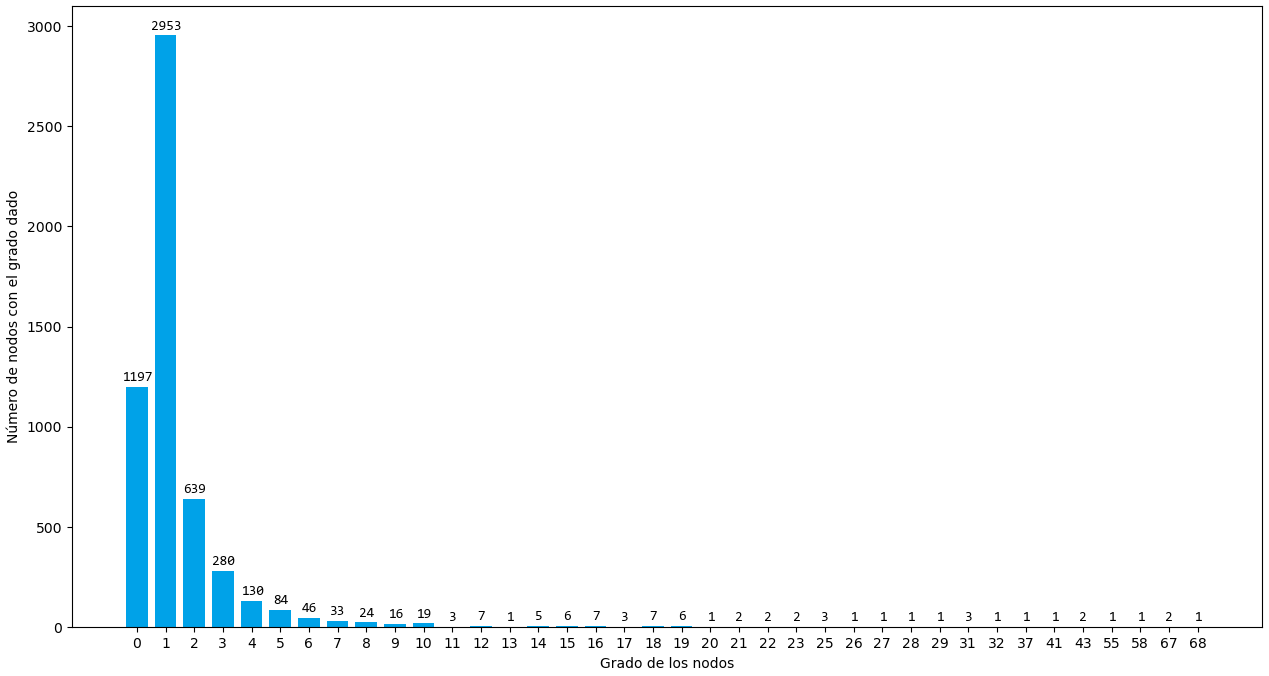
\includegraphics[width=\textwidth]{graphics/degree2.png}
		\caption[Grado de entrada de los nodos del grafo]{Grado de entrada de los nodos del grafo.}
		\label{fig:in_degree_all_nodes}
	\end{center}
\end{figure}

En la figura \ref{fig:out_degree_nodes_by_rol} se evidencia una relación entre el grado de salida de los nodos y la cantidad de estos que tienen un grado específico, pero esta vez agrupados por su rol semántico. Esto representa la cantidad de relaciones como las explicadas en la sección \ref{section:relation_annotation} en las que el nodo es parte izquierda (referenciado a través de \texttt{Arg1}).
\begin{figure}[H]
	\begin{center}
		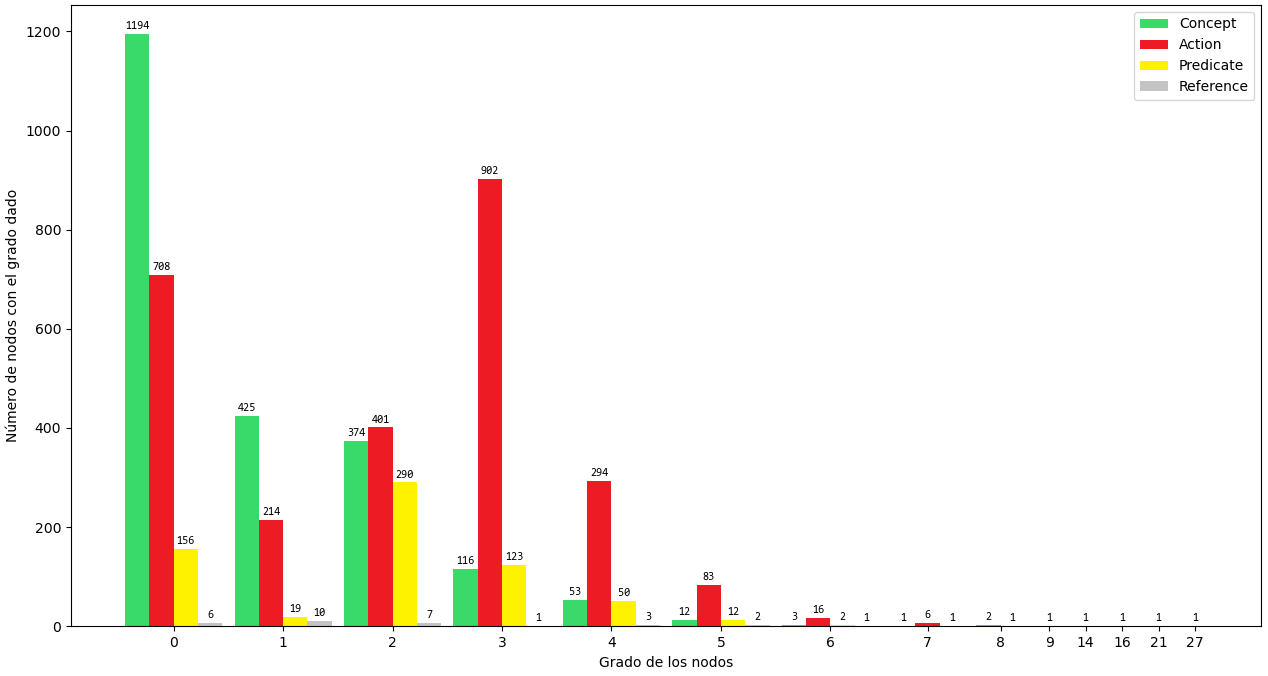
\includegraphics[width=\textwidth]{graphics/degree3.png}
		\caption[Grado de salida de los nodos del grafo por rol]{Grado de salida de los nodos del grafo por rol.}
		\label{fig:out_degree_nodes_by_rol}
	\end{center}
\end{figure}

En la figura \ref{fig:in_degree_nodes_by_rol} se evidencia una relación entre el grado de salida de los nodos y la cantidad de estos que tienen un grado específico, pero esta vez agrupados por su rol semántico. Esto representa la cantidad de relaciones como las explicadas en la sección \ref{section:relation_annotation} en las que el nodo es parte derecha (referenciado a través de \texttt{Arg2}).
\begin{figure}[H]
	\begin{center}
		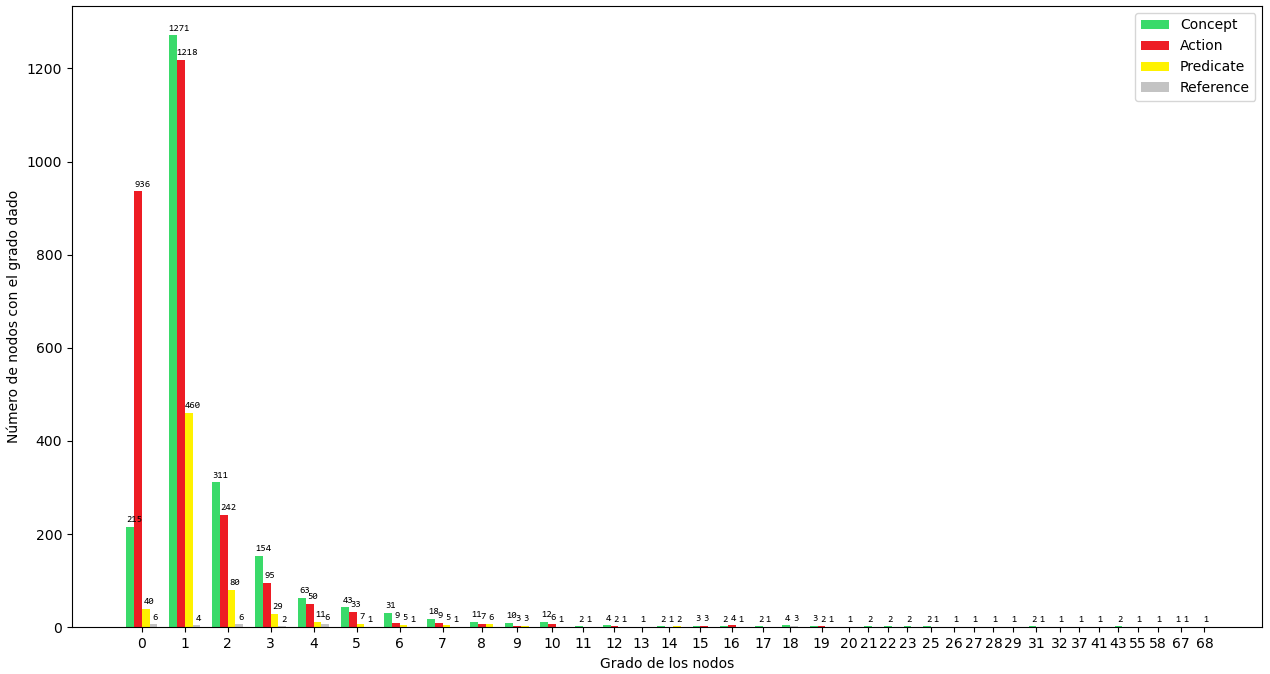
\includegraphics[width=\textwidth]{graphics/degree4.png}
		\caption[Grado de entrada de los nodos del grafo por rol]{Grado de entrada de los nodos del grafo por rol.}
		\label{fig:in_degree_nodes_by_rol}
	\end{center}
\end{figure}

En la tabla \ref{tab:knowledge_graph_stats} se aprecia la cantidad de nodos y aristas según su tipo y a la misma vez se comparan los resultados obtenidos sin normalizar y normalizando las palabras respectivamente. La última columna representa el porcentaje de disminución en cada fila luego de normalizar.
%Esto posibilita una mayor coincidencia de las palabras o frases y por ende, es ideal para una mejor representación y extracción del conocimiento.
\begin{table}[H]
	\begin{center}
		\begin{tabular}{lccc}
			\noalign{\hrule height 1pt}\\
			\vspace{-0.35in}\\
			\textbf{Métrica} & \textbf{Sin normalizar} & \textbf{Normalizando} & \textbf{\% disminuido}\\
			\hline\\
			\vspace{-0.35in}\\
			Conceptos & $5,493$ & $4,935$ & $\approx10.16$\\
			\quad \texttt{Concept} & $2,181$ & $1,969$ & $\approx9.72$\\
			\quad \texttt{Action} & $2,625$ & $2,335$ & $\approx11.05$\\
			\quad \texttt{Reference} & $35$ & $21$ & $40$\\
			\quad \texttt{Predicate} & $652$ & $610$ & $\approx6.44$\\
			\hline\\
			\vspace{-0.35in}\\
			Relaciones & $8,682$ & $8,623$ & $\approx0.68$\\
			\quad \texttt{Concept} & $530$ & $525$ & $\approx0.94$\\
			\quad \texttt{Reference} & $9$ & $9$ & $0$\\
			\quad \texttt{Action} & $1,902$ & $1,875$ & $\approx1.42$\\
			\quad \texttt{Subject} & $923$ & $922$ & $\approx0.11$\\
			\quad \texttt{Target} & $1,572$ & $1,568$ & $\approx0.25$\\
			\quad \texttt{Predicate} & $501$ & $496$ & $\approx1$\\
			\quad \texttt{Domain} & $298$ & $296$ & $\approx0.67$\\
			\quad \texttt{Argument} & $308$ & $307$ & $\approx0.32$\\
			\quad \texttt{Is-a} & $492$ & $481$ & $\approx2.24$\\
			\quad \texttt{Part-of} & $89$ & $89$ & $0$\\
			\quad \texttt{Same-as} & $231$ & $231$ & $0$\\
			\quad \texttt{Has-property} & $143$ & $143$ & $0$\\
			\quad \texttt{Causes} & $360$ & $360$ & $0$\\
			\quad \texttt{Entails} & $200$ & $199$ & $0.5$\\
			\quad \texttt{In-time} & $154$ & $154$ & $0$\\
			\quad \texttt{In-place} & $361$ & $360$ & $\approx0.28$\\
			\quad \texttt{In-context} & $609$ & $608$ & $\approx0.16$\\
			\hline\\
			\vspace{-0.35in}\\
			Atributos & $359$ & $329$ & $\approx8.36$\\
			\quad \texttt{Negated} & $111$ & $94$ & $\approx15.32$\\
			\quad \texttt{Uncertain} & $150$ & $141$ & $6$\\
			\quad \texttt{Diminished} & $83$ & $80$ & $\approx3.61$\\
			\quad \texttt{Emphasized} & $15$ & $14$ & $\approx6.67$\\
			\noalign{\hrule height 1pt}
		\end{tabular}
		\caption[Estadísticas del grafo de conocimiento]{Estadísticas del grafo de conocimiento.}
		\label{tab:knowledge_graph_stats}
	\end{center}
\end{table}

Como se ha podido observar anteriormente, una de las principales funciones de las ontologías y los grafos de conocimiento es la extracción de conocimiento que no está representado explícitamente en el corpus. Un ejemplo de ello es:

\begin{table}[H]
	\begin{center}
		\begin{tabular}{cc}
			\noalign{\hrule height 1pt}\\
			\vspace{-0.35in}\\
			\textbf{Documento} & \textbf{Relación explícita}\\
			\hline\\
			\vspace{-0.35in}\\
			\texttt{cirugía.ann} & \guillemot{\texttt{cirugía de corazón} \textit{is-a} \texttt{operación}}\\
			\texttt{hígado graso.ann} & \guillemot{\texttt{operación} \textit{is-a} \texttt{procedimiento médico}}\\
			\noalign{\hrule height 1pt}\\
			\vspace{-0.35in}\\
			& \textbf{Relación implícita}\\
			& \guillemot{\texttt{cirugía de corazón} \textit{is-a} \texttt{procedimiento médico}}\\
			\noalign{\hrule height 1pt}
		\end{tabular}
		\caption[Ejemplo de extracción de conocimiento implícito]{Ejemplo de extracción de conocimiento implícito.}
		\label{tab:implicit_knowledge_extraction}
	\end{center}
\end{table}

\section{Discusión}
Todos los nodos del grafo de conocimiento participan en al menos una relación, pero como se aprecia en las figuras \ref{fig:out_degree_all_nodes}, \ref{fig:in_degree_all_nodes}, \ref{fig:out_degree_nodes_by_rol} y \ref{fig:in_degree_nodes_by_rol}, hay muchos nodos que tiene un grado bajo. En el caso en que la gráfica muestra la cantidad de nodos con grado cero, esto viene dado o bien porque ese nodo no tiene relaciones de salida y en este caso tendría grado de salida cero o bien no tiene relaciones de entrada y por tanto grado de entrada cero. El hecho de que pocos nodos tengan un alto grado viene dado porque usualmente los nodos más grandes y con más palabras, al ser conocimiento más específico participan en un menor número de relaciones.

Los roles semánticos \textit{Concept} y \textit{Action} que participan en una mayor cantidad de relaciones en este grafo de conocimiento son \guillemot{\texttt{persona}} y \guillemot{\texttt{tratamiento}} respectivamente. Dado que se trabajó con un corpus de documentos médicos, este resultado cobra sentido pues esas palabras son ampliamente empleadas en este medio.

En la tabla \ref{tab:knowledge_graph_stats} se muestra el resultado de un grafo de conocimiento utilizando palabras o frases sin normalizar y normalizadas. Normalizar las palabras no solo reduce la cantidad de nodos y aristas en el grafo sino que también potencialmente aumenta la cantidad de conocimiento implícito que se puede extraer. Esto sucede debido a que en el grafo, todas las relaciones explícitamente escritas en el corpus representan dos nodos y una arista entre estos. Por tanto, si dos nodos no tienen aristas entre ellos, pero existe un camino que los conecta, esto es conocimiento implícito descubierto a través del grafo.

El hecho de normalizar implica, por ejemplo, que todas las conjugaciones de un mismo verbo deben resultar en el verbo sin conjugar. Esto trae consigo muchas ventajas, puesto que todas las relaciones de entrada y salida de ese grupo de palabras quedan contenidas en una única palabra y por ende, puede ampliar potencialmente la cantidad de caminos en el grafo y con ello, la cantidad de conocimiento ímplicito extraído.

Una deficiencia clara sucedió a la hora de hallar los resultados de la tabla \ref{}. Para este tipo de evaluación, lo ideal es tener un grafo de conocimiento formado a partir de una ontología y de un corpus preferentemente grande. A su vez, el grafo debe ser revisado con otro corpus perteneciente al mismo tema y de mediano o gran tamaño. Muchas veces esto es difícil de lograr, y en efecto, es lo que sucedió. Para llevar a cabo esta tarea, se dividieron las oraciones anotadas en dos grupos, un grupo de \textit{training} (\textit{entrenamiento} en español) con el cual se realizará el grafo de conocimiento y un grupo de \textit{testing} (\textit{prueba} en español), con el que se revisará la existencia de las anotaciones de texto y las relaciones respecto a las que ya están construidas en el grafo.

\backmatter

%===================================================================================
% Chapter: Conclusions
%===================================================================================
\Chapter*{Conclusiones}\label{chapter:conclusions}
%===================================================================================

Esta investigación propone un conjunto de elementos orientados al descubrimiento de conocimiento en textos del lenguaje natural. La propuesta se centra en el idioma español y el dominio de la salud, pero es generalizable en ambos aspectos. Entre las contribuciones fundamentales de esta investigación destacan:

\begin{itemize}
	\item[(1)] La definición de un modelo de anotación de propósito general que logra capturar los rasgos semánticos más relevantes contenidos en documentos de texto plano. El mismo es usado como base en la construcción de la ontología propuesta.
	\item[(2)] La definición de un formato de anotación de archivos para el esquema conceptual previamente definido.
	\item[(3)] Se diseñó una propuesta de ontología donde se puede representar un corpus de documentos escritos en lenguaje natural.
	\item[(4)] Se implementó un algoritmo computacional para representar un corpus anotado como grafo de conocimiento a través de dicha ontología.
\end{itemize}

A menudo, una ontología de un dominio no es un objetivo en sí misma. Desarrollarla es similar a definir un conjunto de datos y su estructura para que los utilicen otros programas. Los métodos de resolución de problemas, las aplicaciones independientes del dominio y los usuarios, a menudo las utilizan como datos, en conjunto con bases de conocimiento creadas a partir de las mismas. Por ejemplo, en esta investigación se desarrolla una ontología de dominio médico, la cual se puede utilizar como base para algunas aplicaciones que ofrezcan un conjunto de herramientas de gestión de la salud.

En los resultados se demostró el descubrimiento de conocimiento implícito en el corpus. Esto trae consigo disímiles ventajas, desde el propio descubrimiento de este conocimiento, hasta la interpretación y aprendizaje de un gran número de textos escritos en lenguaje natural, en apenas segundos, mediante el uso de un equipo de cómputo y las propuestas ofrecidas en esta investigación. El conocimiento extraído podría ser usado posteriormente por especialistas en el tema o usuarios, y de esta manera ahorrar el tiempo que tomaría la lectura e interpretación del propio corpus usado para esta tarea.

Teniendo en cuenta que un humano debe tener una gran capacidad de memorización para poder recordar todo lo aprendido en un corpus de documentos, la traba que puede ocasionar tenerlo escrito en un idioma que no se domine, y el factor de no olvidar lo aprendido de él al pasar el tiempo, es clave la utilización de un equipo de cómputo para la creación de la base de conocimiento respectiva al corpus. La misma puede ser fácilmente guardada, leída y usada en el propio sistema o incluso en otros, aportando gran versatilidad al uso de las técnicas mostradas en este estudio.

El descubrimiento automático de conocimiento en el dominio médico tiene especial importancia, pues permitiría identificar interacciones ocultas en la literatura. Además, a pesar de que los recursos médicos disponibles en idioma español son abundantes, los recursos necesarios para la creación de sistemas de extracción automática son más escasos que en otros idiomas, por lo cual la construcción de una ontología y un grafo de conocimiento basado en un corpus del propio dominio, constituyen un hecho relevante para el desarrollo de nuevos sistemas y la continuación de esta investigación en un futuro.
%===================================================================================
% Chapter: Bibliography
%===================================================================================

\bibliographystyle{acm}
\bibliography{bibliography}

\end{document}